\documentclass[11pt]{article}
% ---------------------------------------------------------------------------
% Frenzy and Fade -- research note. Compile with pdfLaTeX + BibTeX (Overleaf default).
% Tables in tables/ and figures in figures/ are generated by make_paper.py.
% ---------------------------------------------------------------------------
\usepackage[T1]{fontenc}
\usepackage[utf8]{inputenc}
\usepackage{mathpazo}
\usepackage[scaled=0.92]{helvet}
\usepackage{microtype}
\usepackage[a4paper,margin=2.4cm]{geometry}
\usepackage{amsmath,amssymb}
\usepackage{booktabs,threeparttable,longtable,array}
\usepackage{graphicx}
\usepackage[font=small,labelfont=bf,labelsep=period,skip=4pt]{caption}
\usepackage{xcolor}
\usepackage{enumitem}
\usepackage[round,authoryear]{natbib}
\usepackage{fancyhdr}
\usepackage{titlesec}
\usepackage[colorlinks=true,linkcolor=accent,citecolor=accent,urlcolor=accent]{hyperref}

\definecolor{accent}{HTML}{1C5CAB}
\definecolor{muted}{HTML}{52514E}
\titleformat{\section}{\normalfont\large\bfseries\color{accent}}{\thesection}{0.8em}{}
\titleformat{\subsection}{\normalfont\normalsize\bfseries}{\thesubsection}{0.8em}{}
\setlength{\parskip}{0.35em}
\setlist{itemsep=0.2em,topsep=0.3em}
\renewcommand{\arraystretch}{1.12}
\pagestyle{fancy}\fancyhf{}
\fancyhead[L]{\small\color{muted}Frenzy and Fade: IPO aftermarket dynamics and cross-asset spillovers}
\fancyhead[R]{\small\color{muted}15 November 2026}
\fancyfoot[C]{\small\thepage}
\renewcommand{\headrulewidth}{0.4pt}

\newcommand{\pct}[1]{#1\%}

\title{\vspace{-1.2em}\textbf{Frenzy and Fade}\\[0.3em]
\large IPO Aftermarket Dynamics, Deal Structure and Cross-Asset Spillovers,\\ with an Application to the Anthropic Listing}
\author{CrossAssetMacro Research}
\date{15 November 2026\\[0.2em]\small Market data to 13 November 2026}

\begin{document}
\maketitle
\thispagestyle{fancy}

\begin{abstract}
\noindent We study the first year of trading of 43 notable US initial public offerings priced between September 2020 and June 2026, and the behaviour of 14 cross-asset series around 11 large listings, to ask whether IPOs follow a ``frenzy then fade'' pattern and what that implies for trading Anthropic, which prices on 18 November 2026. The median IPO rises 19\% on its first day, is roughly flat for a month from the first close, and is 23\% lower by day 126; against the Nasdaq-100 the median shortfall reaches 34\% at day 126 and 39\% at day 252, with bootstrap confidence intervals that exclude zero. Once tests are corrected for multiplicity, only one cross-sectional relationship survives: demand, measured by the final price relative to the first filed range, predicts the first-day return (Spearman $\rho=0.67$, $q<0.001$). Deals priced above their range then give back the most ($-20\%$ by day 63). Market value, sector, listing season, rate regime and the fraction of shares floated produce large differences in medians but none that is statistically reliable. We find no average pre-IPO liquidity drain across asset classes; a softer week after listing and a rebound in the following three weeks do not survive correction. The best historical setup available without an allocation, a conditional fade of above-range deals from day 5, has a per-trade Sharpe ratio of about 0.4. We translate these results into a conditional plan for the Anthropic listing.
\end{abstract}

\noindent\textbf{Keywords:} initial public offerings, aftermarket returns, partial adjustment, event study, multiple testing, cross-asset liquidity.\\
\noindent\textbf{JEL classification:} G12, G14, G24.

\vspace{0.6em}
\noindent\fbox{\parbox{0.97\linewidth}{\small\textbf{Key findings.}
\begin{enumerate}[leftmargin=1.4em]
\item \textbf{The fade is slow, not immediate.} From the first close the median IPO is $+4\%$ at day 5, $-1.5\%$ at day 21 and $-23\%$ at day 126. Relative to QQQ it trails by $34\%$ at day 126 (95\% CI $-46\%$ to $-15\%$).
\item \textbf{Demand predicts the pop and the reversal.} Above-range deals pop $+32\%$ against $+4\%$ and are $-20\%$ at day 63 (CI $-28\%$ to $-2\%$) against $+14\%$. The pop result is the only bucket test that survives a false-discovery-rate correction.
\item \textbf{Buying the open is the weakest entry.} The median debut opens $+23\%$ over the offer and closes $+19\%$; 60\% close below their open; open-to-day-63 is $-11\%$.
\item \textbf{No systematic cross-asset liquidity drain.} Bitcoin, gold and the Nasdaq show no abnormal move before large listings on average; the sell-off before SpaceX and Anthropic is idiosyncratic.
\item \textbf{For Anthropic, condition on the pricing.} Above \$78 places it in the hot-deal group; at or below the range the cohort shows no fade edge. Single-name confidence is low.
\end{enumerate}}}

\section{Introduction}

A large IPO is a liquidity event for its issuer and, increasingly, for the market around it. In 2026 three listings (SpaceX in June, the SK hynix ADR in July and Anthropic in November) will have raised roughly \$160--177bn of equity between them, more than the \$105bn raised by all US IPOs in the second quarter of the year \citep{renaissance2026}. Practitioners describe a recurring pattern: a buying frenzy in the first days, profit-taking, and mean reversion over the following weeks and months, with spillovers to other risk assets as investors raise cash to fund allocations.

This note tests that description on recent data. We make four contributions. First, we measure the post-COVID aftermarket path from the first close, which is the price a non-allocated buyer actually pays, with bootstrap confidence intervals and market-adjusted versions. Second, we bucket the cohort by market value, sector, listing season, macro regime, float and demand, and test each split with a correction for the number of tests run. Third, we study the intraday shape of debut sessions using daily and hourly bars. Fourth, we run an event study of 14 cross-asset series around 11 large listings, at daily and hourly frequency, against a random-date baseline. We then convert the results into trade-level statistics, including implied Sharpe ratios, and apply them to Anthropic.

The results connect to a long literature. Long-run underperformance of IPOs is documented by \citet{ritter1991} and \citet{loughran1995}; the link between price revisions during bookbuilding and first-day returns is the partial-adjustment effect of \citet{hanley1993}; lock-up expirations carry negative abnormal returns \citep{field2001,aggarwal2002}; and IPO activity and initial returns are clustered in time \citep{lowry2002}. \citet{ljungqvist2007} surveys underpricing. Our sample is small and recent, so our emphasis is on what survives formal inference rather than on point estimates.

\section{Data}

\paragraph{IPO cohort.} The sample (Table~\ref{tab:sample}; full list in Appendix Table~\ref{tab:cohort}) contains 43 notable US IPOs from Snowflake (September 2020) to SpaceX (June 2026). It is hand-selected, which biases it toward large, well-known deals, and it contains no 2022 listings because that window was effectively closed. Direct listings are excluded because they have no underwritten offer price, and the SK hynix ADR is excluded from IPO-level statistics because it is a cross-listing of an already public company.

\paragraph{Deal terms.} Offer price, shares offered, gross proceeds, the first and final filed price ranges, upsizing and shares outstanding come from SEC 424B4 prospectuses and company pricing releases. Float is gross proceeds divided by market value at the offer price. Oversubscription multiples are published for only two deals (Reddit, 5$\times$; Gemini, 20$\times$), so we follow the literature and proxy demand by the offer price relative to the first filed range.

\paragraph{Prices and macro data.} Daily open, high, low and close and 60-minute bars are from Yahoo Finance; the hourly feed covers only the last two years, and we keep the 14 IPOs since January 2025 whose hourly data include the debut session. Cross-asset series are SPY, QQQ, IWM, ARKK, SMH, IGV, Bitcoin, GLD, TLT, UUP, HYG, the VIX, the 10-year Treasury yield and the Renaissance IPO ETF. Effective fed funds and the components of Fed net liquidity are from FRED.

\begin{table}[!htbp]\centering\small
\caption{Sample description}\label{tab:sample}

\begin{threeparttable}
\begin{tabular}{lr}
\toprule
& Value \\
\midrule
IPOs in sample & 43 \\
Listing window & 2020-09-16 to 2026-06-12 \\
Median market value at offer (\$bn) & 9.2 \\
Median gross proceeds (\$m) & 1,205 \\
Median float (proceeds / market value) & 12.8\% \\
Priced above first filed range & 28 of 42 \\
Upsized & 9 \\
Median / mean first-day return & +19.2\% / +37.1\% \\
\midrule
\multicolumn{2}{l}{\textit{Sector composition}} \\
\quad Software, AI \& semis & 12 \\
\quad Fintech \& financials & 9 \\
\quad Consumer internet & 8 \\
\quad Industrials, energy \& space & 6 \\
\quad Healthcare & 4 \\
\quad Consumer \& leisure & 4 \\
\midrule
\multicolumn{2}{l}{\textit{Market value at offer}} \\
\quad Small $<$10B & 22 \\
\quad Mid 10-30B & 11 \\
\quad Large 30-100B & 9 \\
\quad Mega $\geq$100B & 1 \\
\bottomrule
\end{tabular}
\begin{tablenotes}[flushleft]\footnotesize
\item \textit{Notes:} Hand-selected notable US IPOs priced between September 2020 and June 2026. Deal terms from SEC 424B4 prospectuses and pricing releases. Direct listings and the SK hynix ADR cross-listing are excluded from IPO-level statistics.
\end{tablenotes}
\end{threeparttable}

\end{table}


\section{Methodology}

\paragraph{Returns.} Day 1 is the first trading close. The first-day return is $r^{\text{pop}}_i = P_{i,1}/O_i - 1$, where $O_i$ is the offer price. Aftermarket returns are measured from the first close, $r_{i}(h) = P_{i,h}/P_{i,1} - 1$, at $h \in \{5, 21, 63, 126, 252\}$ trading days. Market-adjusted returns subtract the QQQ return over the same dates.

\paragraph{Inference.} For a statistic $\hat\theta$ (mean or median across IPOs) we report 95\% bootstrap percentile intervals from 10,000 resamples of IPOs \citep{efron1993}. Single strategies are tested with a one-sample $t$-test on the mean and a Wilcoxon signed-rank test on the median. Differences across buckets use the Kruskal--Wallis test; associations use Spearman's $\rho$. Because we run many tests, we report Benjamini--Hochberg $q$-values \citep{benjamini1995} within each family: 28 bucket tests, 11 correlations and 56 cross-asset windows.

\paragraph{Cross-asset event study.} For each asset and window $[a,b]$ relative to the listing day we compute the average move across the 11 events, $\bar r_{[a,b]}$. Its null distribution is built by drawing 11 random dates 10,000 times from all trading days since June 2020 and averaging the same window; the two-sided $p$-value is the share of draws at least as far from the null mean as the observed average. We also report the leave-one-out range of the excess move. At hourly frequency, the abnormal return of an asset in the hour an IPO opens is its return in that bar minus the mean of the same clock hour over the prior 20 sessions.

\paragraph{Sharpe ratios.} For a strategy with per-trade returns $x_1,\dots,x_n$ and holding period $h$ days,
\begin{equation}
\mathrm{SR}_{\text{trade}} = \frac{\bar x}{s_x}, \qquad \mathrm{SR}_{\text{ann}} = \mathrm{SR}_{\text{trade}}\sqrt{252/h}, \qquad \mathrm{SR}_{\text{real}} = \mathrm{SR}_{\text{trade}}\sqrt{N},
\end{equation}
where $N$ is the number of comparable setups per year (7.5 IPOs in our cohort; 1.8 large listings). $\mathrm{SR}_{\text{ann}}$ assumes the trade can be repeated back to back and is an upper bound; $\mathrm{SR}_{\text{real}}$ assumes cash between setups and is the relevant figure for a strategy that waits for IPOs. We label a strategy \emph{High} confidence if its CI excludes zero and $p_W<0.05$, \emph{Medium} if $\min(p_t,p_W)<0.10$, and \emph{Low} otherwise.

\section{Results}

\subsection{The aftermarket path}

Table~\ref{tab:horizons} and Figure~\ref{fig:path} show the central fact. The median first-day return is 19\% (mean 37\%, reflecting a few very large pops). From the first close, the median IPO gains 4\% in the first week, is roughly flat at one month ($-1.5\%$), and is 7\% lower at three months and 23\% lower at six months. The raw band excludes zero only between about months four and seven. Market-adjusted, the picture is sharper: the median IPO trails QQQ by 14\% at day 63, 34\% at day 126 (CI $-46\%$ to $-15\%$) and 39\% at day 252 (CI $-48\%$ to $-10\%$). Means are much higher than medians at long horizons because the distribution is right-skewed; CoreWeave alone gained roughly 300\% in its first three months.

\begin{figure}[!htbp]\centering
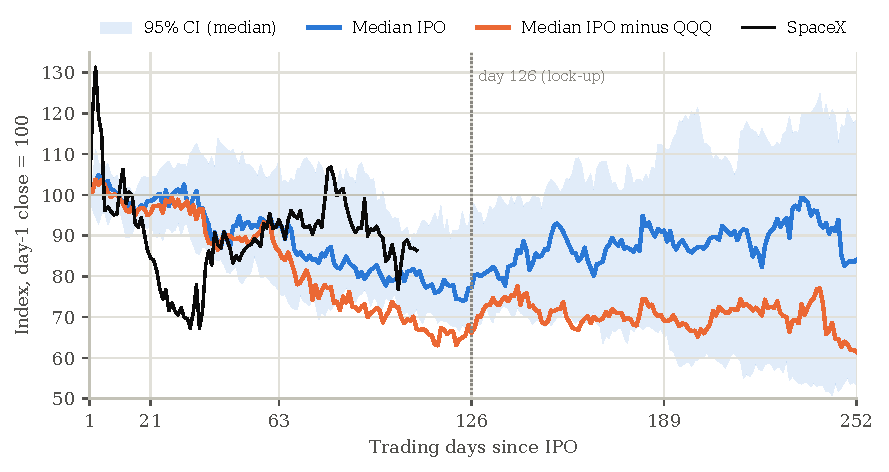
\includegraphics[width=\linewidth]{figures/f1_path.pdf}
\caption{Median price path from the first close, 43 IPOs. The shaded band is the 95\% bootstrap CI of the median, shown while at least eight IPOs remain. SpaceX is plotted for comparison.}\label{fig:path}
\end{figure}

\begin{table*}[!htbp]\centering\small
\caption{Aftermarket returns by horizon}\label{tab:horizons}
\resizebox{\linewidth}{!}{
\begin{threeparttable}
\begin{tabular}{lrrrcrrc}
\toprule
Window & $n$ & Mean & Median & 95\% CI (median) & \% $<0$ & Med.\ vs QQQ & 95\% CI \\
\midrule
Offer to day-1 close (first-day return) & 43 & +37.1 & +19.2 & [+12, +32] & 16 & -- & -- \\
Day-1 close to day 5 & 43 & +5.3 & +4.2 & [$-$5, +7] & 42 & +3.7 & [$-$7, +5] \\
Day-1 close to day 21 & 43 & +2.5 & $-$1.5 & [$-$7, +5] & 53 & $-$4.5 & [$-$11, +4] \\
Day-1 close to day 63 & 43 & +2.7 & $-$7.0 & [$-$24, +8] & 58 & $-$13.8 & [$-$29, +1] \\
Day-1 close to day 126 & 42 & $-$11.7 & $-$22.7 & [$-$31, $-$2] & 64 & $-$33.8 & [$-$46, $-$15] \\
Day-1 close to day 252 & 41 & +0.2 & $-$15.9 & [$-$47, +18] & 56 & $-$38.6 & [$-$48, $-$10] \\
\bottomrule
\end{tabular}
\begin{tablenotes}[flushleft]\footnotesize
\item \textit{Notes:} Returns in percent. Horizons are trading days counted from the first close (day 1). ``vs QQQ'' subtracts the QQQ return over the same dates. Confidence intervals are 10,000-draw bootstrap percentile intervals of the median.
\end{tablenotes}
\end{threeparttable}
}
\end{table*}


Day-by-day returns (Table~\ref{tab:daily}) show momentum on days 2 and 3 (mean $+1.6\%$ and $+2.6\%$) and a reversal on day 6 ($-2.6\%$, $p=0.03$), but none of these survives a correction for testing nine days. The frenzy is visible in the averages; it is not statistically reliable at the daily level.

\begin{table}[!htbp]\centering\small
\caption{Close-to-close returns, days 2 to 10}\label{tab:daily}

\begin{threeparttable}
\begin{tabular}{lrcrrrr}
\toprule
Day & Mean & 95\% CI & Median & \% up & $p$ ($t$-test) & Mean vs QQQ \\
\midrule
Day 2 & +1.63 & [$-$1.30, +4.78] & +0.95 & 58 & 0.31 & +1.57 \\
Day 3 & +2.63 & [$-$0.48, +5.94] & +3.75 & 67 & 0.12 & +2.23 \\
Day 4 & $-$0.94 & [$-$3.20, +1.56] & $-$2.68 & 28 & 0.45 & $-$0.80 \\
Day 5 & +1.40 & [$-$1.15, +4.64] & $-$0.20 & 47 & 0.35 & +1.11 \\
Day 6 & $-$2.57 & [$-$4.89, $-$0.39] & $-$1.42 & 35 & 0.032$^{**}$ & $-$2.23 \\
Day 7 & +0.81 & [$-$0.92, +2.69] & $-$0.17 & 47 & 0.39 & +0.76 \\
Day 8 & +0.62 & [$-$0.94, +2.19] & $-$0.07 & 49 & 0.45 & +0.54 \\
Day 9 & $-$0.11 & [$-$1.54, +1.35] & $-$0.47 & 44 & 0.88 & $-$0.38 \\
Day 10 & $-$0.45 & [$-$2.35, +1.80] & $-$0.44 & 44 & 0.68 & $-$0.16 \\
\bottomrule
\end{tabular}
\begin{tablenotes}[flushleft]\footnotesize
\item \textit{Notes:} Percent. 43 IPOs. Stars: $^{*}p<0.10$, $^{**}p<0.05$, $^{***}p<0.01$ (unadjusted). With nine days tested, the day-6 result does not survive a Bonferroni or Benjamini--Hochberg correction.
\end{tablenotes}
\end{threeparttable}

\end{table}


\subsection{Market value, sector, season and macro regime}

Tables~\ref{tab:buckets} and~\ref{tab:regimes} split the cohort. The medians differ a lot: consumer internet faded first ($-25\%$ at day 63), fintech and crypto faded hardest ($-41\%$ at day 126), and software, AI and semiconductors held up best ($-3\%$ at day 63; Figure~\ref{fig:sectors}). Q4 and Q1 listings had the largest pops ($+39\%$ and $+34\%$) and Q3 listings the weakest six months ($-33\%$). IPOs that listed after a three-month rise of more than 30bp in the 10-year yield had a median day-63 return of $-18\%$ against $+2\%$ with flat yields, and high volatility at listing (VIX above 22) came with the largest pops ($+56\%$).

None of these differences is statistically reliable. Every Kruskal--Wallis $q$-value for market value, sector, quarter, rates and VIX is 0.57 or higher. With 4 to 30 IPOs per bucket the confidence intervals overlap heavily. These splits are useful as priors, not as signals.

\begin{table}[!htbp]\centering\footnotesize
\caption{Median returns by market value, sector and listing quarter}\label{tab:buckets}

\begin{threeparttable}
\begin{tabular}{lrrrrcr}
\toprule
& $n$ & Pop & Day 21 & Day 63 & 95\% CI (day 63) & Day 126 \\
\midrule
\multicolumn{7}{l}{\textit{Panel A. Market value at offer}} \\
\quad Small $<$10B & 22 & +17 & +1 & $-$5 & [$-$22, +18] & $-$21 \\
\quad Mid 10-30B & 11 & +12 & $-$3 & $-$27 & [$-$35, +37] & $-$26 \\
\quad Large 30-100B & 9 & +41 & $-$4 & +2 & [$-$36, +30] & $-$24 \\
\quad Mega $\geq$100B & 1 & +19 & $-$15 & $-$6 & [--, --] & -- \\
\quad \footnotesize Kruskal--Wallis $p$ ($q$) & & \footnotesize 0.47 (0.88) & \footnotesize 0.79 (0.91) & \multicolumn{2}{c}{\footnotesize 0.79 (0.91)} & \footnotesize 0.79 (0.91) \\
\addlinespace
\multicolumn{7}{l}{\textit{Panel B. Sector}} \\
\quad Consumer \& leisure & 4 & +10 & +9 & 0 & [$-$34, +37] & +2 \\
\quad Consumer internet & 8 & +45 & $-$10 & $-$25 & [$-$35, +14] & $-$28 \\
\quad Fintech \& financials & 9 & +14 & +21 & $-$27 & [$-$35, +30] & $-$41 \\
\quad Healthcare & 4 & +13 & +4 & +27 & [+6, +49] & +11 \\
\quad Industrials, energy \& space & 6 & +23 & $-$4 & $-$15 & [$-$50, +3] & $-$26 \\
\quad Software, AI \& semis & 12 & +28 & $-$6 & $-$3 & [$-$14, +35] & $-$15 \\
\quad \footnotesize Kruskal--Wallis $p$ ($q$) & & \footnotesize 0.63 (0.91) & \footnotesize 0.10 (0.57) & \multicolumn{2}{c}{\footnotesize 0.21 (0.57)} & \footnotesize 0.18 (0.57) \\
\addlinespace
\multicolumn{7}{l}{\textit{Panel C. Listing quarter}} \\
\quad Q1 & 10 & +34 & $-$4 & $-$18 & [$-$30, +11] & $-$29 \\
\quad Q2 & 12 & +14 & +5 & $-$4 & [$-$26, +34] & +2 \\
\quad Q3 & 15 & +18 & $-$5 & $-$11 & [$-$28, +14] & $-$33 \\
\quad Q4 & 6 & +39 & +4 & $-$9 & [$-$30, +31] & $-$17 \\
\quad \footnotesize Kruskal--Wallis $p$ ($q$) & & \footnotesize 0.68 (0.91) & \footnotesize 0.43 (0.87) & \multicolumn{2}{c}{\footnotesize 0.82 (0.91)} & \footnotesize 0.33 (0.76) \\
\addlinespace
\bottomrule
\end{tabular}
\begin{tablenotes}[flushleft]\footnotesize
\item \textit{Notes:} Medians in percent. Pop is the first-day return from the offer; later columns are measured from the day-1 close. $q$ = Benjamini--Hochberg adjusted across all 28 bucket tests in Tables~\ref{tab:buckets} and \ref{tab:regimes}.
\end{tablenotes}
\end{threeparttable}

\end{table}


\begin{figure}[!htbp]\centering
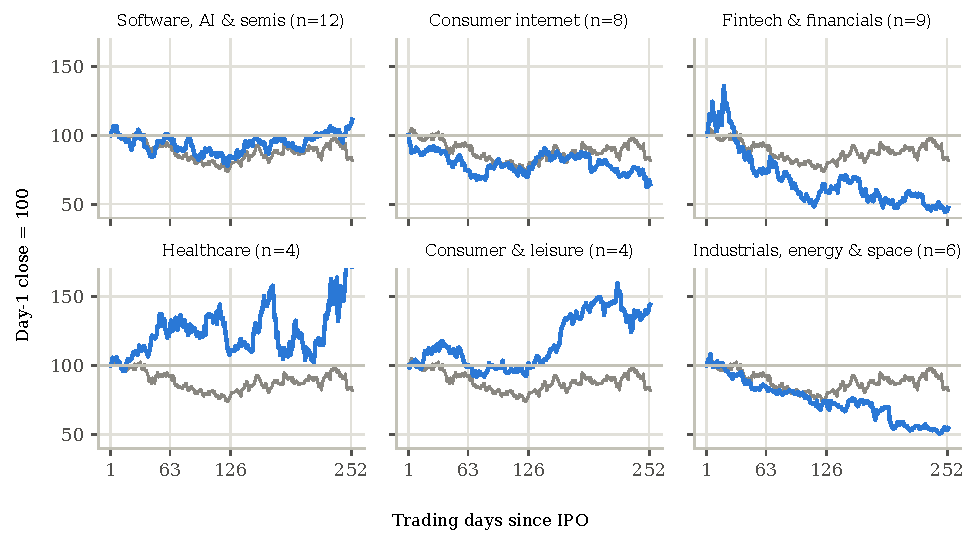
\includegraphics[width=\linewidth]{figures/f2_sectors.pdf}
\caption{Median path from the first close by sector (blue) against all IPOs (grey).}\label{fig:sectors}
\end{figure}

\begin{table}[!htbp]\centering\footnotesize
\caption{Median returns by macro regime and deal structure}\label{tab:regimes}

\begin{threeparttable}
\begin{tabular}{lrrrrcr}
\toprule
& $n$ & Pop & Day 21 & Day 63 & 95\% CI (day 63) & Day 126 \\
\midrule
\multicolumn{7}{l}{\textit{Panel A. 10-year yield, 3-month change before listing}} \\
\quad 10Y falling & 10 & +16 & $-$1 & $-$7 & [$-$30, +20] & $-$46 \\
\quad 10Y flat & 18 & +34 & +1 & +2 & [$-$28, +35] & $-$10 \\
\quad 10Y rising & 15 & +12 & $-$6 & $-$18 & [$-$27, +2] & $-$20 \\
\quad \footnotesize Kruskal--Wallis $p$ ($q$) & & \footnotesize 0.15 (0.57) & \footnotesize 0.69 (0.91) & \multicolumn{2}{c}{\footnotesize 0.41 (0.87)} & \footnotesize 0.20 (0.57) \\
\addlinespace
\multicolumn{7}{l}{\textit{Panel B. VIX level at listing}} \\
\quad VIX $<$16 & 17 & +14 & $-$6 & $-$11 & [$-$27, +14] & $-$6 \\
\quad VIX 16-22 & 19 & +19 & +5 & $-$2 & [$-$33, +14] & $-$27 \\
\quad VIX $>$22 & 7 & +56 & $-$4 & $-$23 & [$-$29, +43] & $-$36 \\
\quad \footnotesize Kruskal--Wallis $p$ ($q$) & & \footnotesize 0.15 (0.57) & \footnotesize 0.21 (0.57) & \multicolumn{2}{c}{\footnotesize 0.92 (0.97)} & \footnotesize 0.55 (0.91) \\
\addlinespace
\multicolumn{7}{l}{\textit{Panel C. Float (proceeds / market value)}} \\
\quad Float $<$8\% & 13 & +19 & $-$7 & $-$14 & [$-$35, +23] & $-$24 \\
\quad Float 8-15\% & 17 & +18 & $-$4 & $-$11 & [$-$28, +8] & $-$25 \\
\quad Float $>$15\% & 13 & +27 & +5 & +6 & [$-$27, +19] & $-$12 \\
\quad \footnotesize Kruskal--Wallis $p$ ($q$) & & \footnotesize 0.97 (0.97) & \footnotesize 0.22 (0.57) & \multicolumn{2}{c}{\footnotesize 0.77 (0.91)} & \footnotesize 0.63 (0.91) \\
\addlinespace
\multicolumn{7}{l}{\textit{Panel D. Final price vs first filed range}} \\
\quad At or below initial range & 14 & +4 & +1 & +14 & [$-$14, +30] & +7 \\
\quad Priced above initial range & 28 & +32 & $-$2 & $-$20 & [$-$28, $-$2] & $-$27 \\
\quad \footnotesize Kruskal--Wallis $p$ ($q$) & & \footnotesize 0.001 (0.040) & \footnotesize 0.94 (0.97) & \multicolumn{2}{c}{\footnotesize 0.11 (0.57)} & \footnotesize 0.037 (0.52) \\
\addlinespace
\bottomrule
\end{tabular}
\begin{tablenotes}[flushleft]\footnotesize
\item \textit{Notes:} As Table~\ref{tab:buckets}. 10Y rising/falling: more than $\pm$30bp over the three months before listing. Demand proxy: offer price relative to the first filed range \citep{hanley1993}; only 3 deals priced below range, so they are pooled with within-range deals.
\end{tablenotes}
\end{threeparttable}

\end{table}


The market-level seasonal evidence is stronger because it rests on 76 years of data (Figure~\ref{fig:season}). November and December are two of the three best months for the S\&P~500 since 1950 (average $+1.8\%$ and $+1.4\%$). From 15 November of a midterm-election year the index rose over the next three months in 18 of 19 cases, with an average gain of 7.7\%, against 2.3\% and a 63\% hit rate in other years.

\begin{figure}[!htbp]\centering
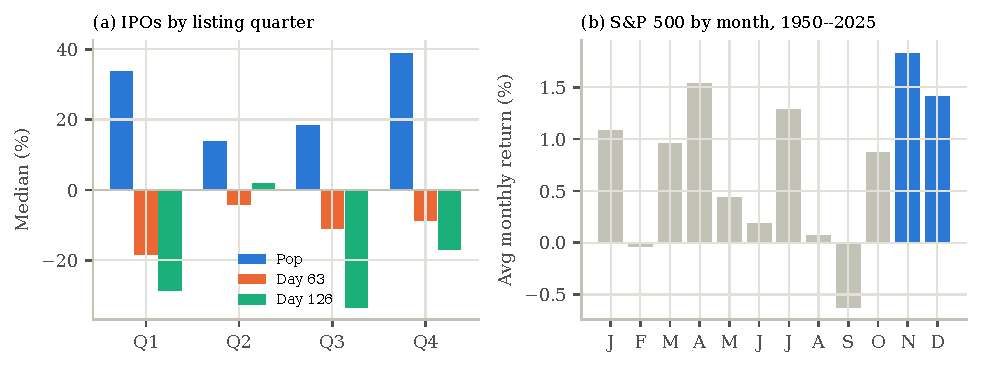
\includegraphics[width=\linewidth]{figures/f8_season.pdf}
\caption{(a) Median IPO outcomes by listing quarter. (b) Average S\&P~500 monthly return, 1950--2025; November and December highlighted.}\label{fig:season}
\end{figure}

\subsection{Deal structure: float and demand}

Demand is the one dimension that matters (Figure~\ref{fig:demand}; Table~\ref{tab:regimes}, Panel~D). Deals priced above their first filed range had a median first-day return of 32\% (CI 17\% to 60\%) against 4\% for deals priced within or below it; the Kruskal--Wallis test gives $p=0.001$, $q=0.04$, and the rank correlation between the price revision and the pop is 0.67 ($q<0.001$; Table~\ref{tab:corr}). This is the partial-adjustment effect of \citet{hanley1993}: issuers raise the price when the book is strong but leave money on the table.

The same hot deals then gave back the most. Their median day-63 return from the first close was $-20\%$ (CI $-28\%$ to $-2\%$) against $+14\%$, and their day-126 return was $-27\%$ against $+7\%$. The day-126 difference is significant on its own ($p=0.037$) but not after correction ($q=0.52$). The fraction of shares floated, by contrast, shows no relationship with the pop or the aftermarket (all $p>0.2$). Low-float deals such as Anthropic's (about 4.5\%) are not systematically different from the rest of the cohort.

\begin{figure}[!htbp]\centering
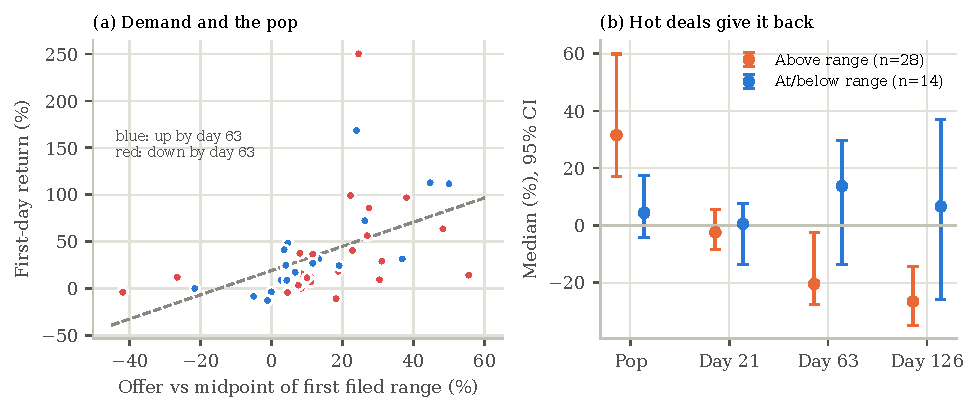
\includegraphics[width=\linewidth]{figures/f3_demand.pdf}
\caption{(a) Price revision against the first-day return; colour shows the sign of the day-63 return. (b) Medians and 95\% CIs for deals priced above their first filed range and for the rest.}\label{fig:demand}
\end{figure}

\begin{table}[!htbp]\centering\small
\caption{Spearman rank correlations}\label{tab:corr}

\begin{threeparttable}
\begin{tabular}{lrrrr}
\toprule
Pair & $n$ & $\rho$ & $p$ & $q$ (BH) \\
\midrule
Day-1 pop vs day-21 return & 43 & $+$0.04 & 0.80 & 0.88 \\
Day-1 pop vs day-63 return & 43 & $+$0.01 & 0.96 & 0.96 \\
Opening pop vs open-to-close & 43 & $+$0.07 & 0.66 & 0.80 \\
Market cap vs day-1 pop & 43 & $+$0.11 & 0.49 & 0.80 \\
10Y 3-month change vs day-63 return & 43 & $-$0.14 & 0.37 & 0.80 \\
VIX vs day-1 pop & 43 & $+$0.23 & 0.13 & 0.74 \\
Day 1-5 squeeze vs day 5-63 return (non-overlapping) & 43 & $+$0.09 & 0.57 & 0.80 \\
Float \% vs day-1 pop & 43 & $-$0.08 & 0.61 & 0.80 \\
Float \% vs day-63 return & 43 & $+$0.13 & 0.42 & 0.80 \\
Price revision vs day-1 pop & 42 & $+$0.67 & $<$0.001 & $<$0.001 \\
Price revision vs day-63 return & 42 & $-$0.15 & 0.35 & 0.80 \\
\bottomrule
\end{tabular}
\begin{tablenotes}[flushleft]\footnotesize
\item \textit{Notes:} Returns measured from the day-1 close unless stated. The squeeze test uses non-overlapping windows (days 1--5 vs days 5--63). $q$ adjusts across the 11 correlations.
\end{tablenotes}
\end{threeparttable}

\end{table}


\subsection{Intraday dynamics}

Table~\ref{tab:intraday} uses daily open, high and close for all 43 debuts. The median IPO opens 23\% above its offer, closes 19\% above, and ends the day 7.5\% below its high; 60\% close below their opening price. Buying the open and selling the close lost 1.1\% on average (CI $-4.3\%$ to $+2.2\%$), and buying the open and holding to day 63 lost a median 11\%. The size of the opening pop does not predict the rest of the session (Spearman $\rho=0.07$, $p=0.66$).

Hourly bars for the 14 IPOs since January 2025 show the mechanics (Table~\ref{tab:hourly}; Figure~\ref{fig:intraday}). The first print typically comes late, with a median first bar of 12:30 ET. Volume is concentrated in the first hour or two after the opening print (roughly 40\% of the session in each of the 11:30 and 12:30 bars). The high of the day came in that first trading hour for 10 of the 14 IPOs. Most day-1 hourly bars after the open have negative median returns. On day 2 the first hourly bar is the only clearly negative one: its median return is $-1.8\%$ and it was down for 79\% of the IPOs. SpaceX (panel b) is a clean example: it opened at 11:30 ET, closed day 1 up 19\%, peaked on day 3, and a $-9\%$ reversal on day 4 began a fade that took it below its offer by day 23.

\begin{table*}[!htbp]\centering\small
\caption{Debut-day shape by size of the opening print}\label{tab:intraday}
\resizebox{\linewidth}{!}{
\begin{threeparttable}
\begin{tabular}{lrrrrrrrr}
\toprule
Opening print vs offer & $n$ & Open & Close & Open$\to$close & Close vs high & \% below open & Open$\to$D21 & Open$\to$D63 \\
\midrule
Open $<$10\% over offer & 12 & 0 & $-$2 & $-$0.8 & $-$4.3 & 58 & +2.4 & +9.7 \\
Open 10-40\% & 17 & +23 & +17 & $-$5.1 & $-$8.8 & 71 & $-$9.3 & $-$20.1 \\
Open $>$40\% & 14 & +80 & +79 & +1.4 & $-$11.3 & 50 & +0.4 & $-$17.2 \\
\midrule
All IPOs & 43 & +23 & +19 & $-$2.0 & $-$7.5 & 60 & $-$1.6 & $-$10.8 \\
\bottomrule
\end{tabular}
\begin{tablenotes}[flushleft]\footnotesize
\item \textit{Notes:} Medians in percent from daily open, high and close. The last two columns measure returns from the opening price, the entry available to a buyer without an allocation.
\end{tablenotes}
\end{threeparttable}
}
\end{table*}

\begin{table}[!htbp]\centering\small
\caption{Hourly profile of the first three sessions}\label{tab:hourly}

\begin{threeparttable}
\begin{tabular}{lrrrrrr}
\toprule
Bar (ET) & \multicolumn{3}{c}{Share of day's volume (\%)} & \multicolumn{3}{c}{Median bar return (\%)} \\ \cmidrule(lr){2-4}\cmidrule(lr){5-7} & Day 1 & Day 2 & Day 3 & Day 1 & Day 2 & Day 3 \\
\midrule
9:30 & -- & 35 & 37 & -- & $-$1.8 & +3.8 \\
10:30 & -- & 16 & 15 & -- & +1.1 & +0.6 \\
11:30 & 38 & 9 & 11 & $-$2.5 & $-$0.2 & $-$0.4 \\
12:30 & 40 & 8 & 8 & $-$2.2 & +0.5 & +0.2 \\
13:30 & 18 & 8 & 6 & $-$0.1 & +0.7 & $-$0.1 \\
14:30 & 16 & 7 & 10 & $-$2.6 & +0.1 & $-$0.1 \\
15:30 & 12 & 10 & 12 & $-$0.1 & $-$0.2 & $-$0.4 \\
\bottomrule
\end{tabular}
\begin{tablenotes}[flushleft]\footnotesize
\item \textit{Notes:} 14 IPOs since January 2025 whose hourly feed includes the debut session. Day-1 bars with fewer than four IPOs trading are omitted (most debuts open between 11:30 and 13:30 ET). The debut-day high fell in the first trading hour for 10 of 14 IPOs.
\end{tablenotes}
\end{threeparttable}

\end{table}


\begin{figure}[!htbp]\centering
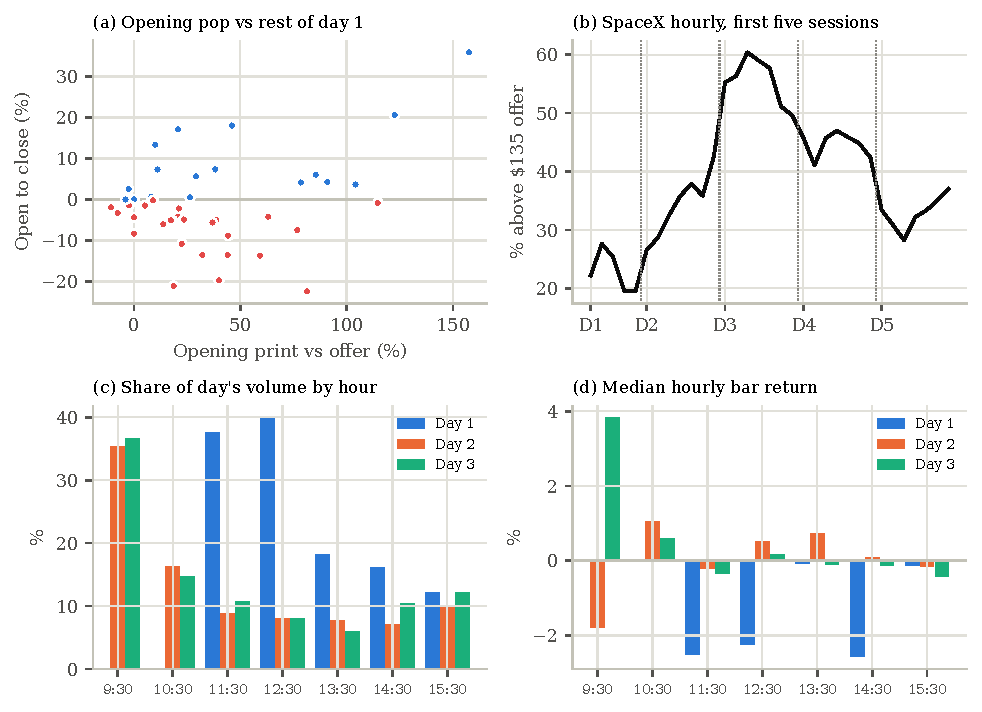
\includegraphics[width=\linewidth]{figures/f4_intraday.pdf}
\caption{Intraday evidence. (a) Opening pop against the open-to-close return, 43 IPOs. (b) SpaceX hourly closes over its first five sessions. (c) Median share of the session's volume by hourly bar. (d) Median hourly bar return.}\label{fig:intraday}
\end{figure}

\subsection{Trading strategies and implied Sharpe ratios}

Table~\ref{tab:strategies} and Figure~\ref{fig:forest} evaluate simple strategies on the IPO stock. Only the allocation flip, buying at the offer and selling at the first close, is unambiguously profitable: $+37\%$ per trade on average (CI $+23\%$ to $+54\%$), positive 79\% of the time, with a per-trade Sharpe ratio of 0.72. That return is available only to investors who are allocated, and allocations in hot deals are small.

For a trader without an allocation, every unconditional strategy is weak. The squeeze (long from the first close to day 5) earns $+5\%$ on average but with a CI that includes zero. Shorting from day 5 to day 63 is positive in the median ($+14\%$) but not in the mean, because a few large winners dominate. Market-adjusted, the short from day 5 to day 63 has a median of $+17\%$ and a Wilcoxon $p$ of 0.03 (Medium confidence). Its per-trade Sharpe is only 0.19, about 0.5 a year at 7.5 setups.

Conditioning helps (Table~\ref{tab:subsets}). For deals priced above their first range, the short from day 5 to day 63 earned $+11.5\%$ on average with a 71\% hit rate and $p_W=0.03$, a per-trade Sharpe of 0.37. This is the best non-allocated setup in the data, and it is consistent with the demand results above.

\begin{figure}[!htbp]\centering
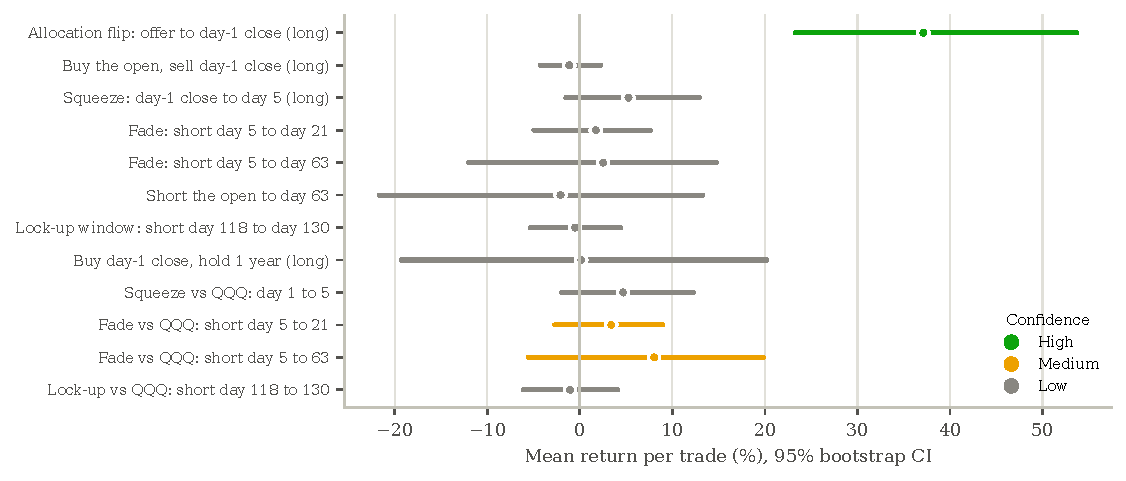
\includegraphics[width=\linewidth]{figures/f5_forest.pdf}
\caption{Mean return per trade with 95\% bootstrap CI for each strategy; colour gives the confidence label defined in Section~3.}\label{fig:forest}
\end{figure}

\begin{table*}[!htbp]\centering\scriptsize
\caption{Trading strategies on the IPO stock: returns, significance and implied Sharpe ratios}\label{tab:strategies}
\resizebox{\linewidth}{!}{
\begin{threeparttable}
\begin{tabular}{lrrcrrrrrrrl}
\toprule
Strategy & $n$ & Mean & 95\% CI & Median & Hit & $p_t$ & $p_W$ & SR$_\text{trade}$ & SR$_\text{ann}$ & SR$_\text{real}$ & Conf. \\
\midrule
Allocation flip: offer to day-1 close (long) & 43 & +37.1 & [+23, +54] & +19.2 & 79 & $<$0.001 & $<$0.001 & 0.72 & 11.44 & 1.97 & High \\
Buy the open, sell day-1 close (long) & 43 & $-$1.1 & [$-$4, +2] & $-$2.0 & 35 & 0.50 & 0.19 & $-$0.10 & $-$1.63 & $-$0.28 & Low \\
Squeeze: day-1 close to day 5 (long) & 43 & +5.3 & [$-$1, +13] & +4.2 & 58 & 0.16 & 0.54 & 0.22 & 1.71 & 0.59 & Low \\
Fade: short day 5 to day 21 & 43 & +1.7 & [$-$5, +8] & +2.4 & 60 & 0.59 & 0.22 & 0.08 & 0.33 & 0.23 & Low \\
Fade: short day 5 to day 63 & 43 & +2.5 & [$-$12, +15] & +14.3 & 65 & 0.71 & 0.17 & 0.06 & 0.12 & 0.15 & Low \\
Short the open to day 63 & 43 & $-$2.1 & [$-$22, +13] & +10.8 & 56 & 0.82 & 0.39 & $-$0.03 & $-$0.07 & $-$0.09 & Low \\
Lock-up window: short day 118 to day 130 & 42 & $-$0.5 & [$-$5, +4] & +0.5 & 50 & 0.84 & 0.79 & $-$0.03 & $-$0.14 & $-$0.09 & Low \\
Buy day-1 close, hold 1 year (long) & 41 & +0.2 & [$-$19, +20] & $-$15.9 & 44 & 0.99 & 0.90 & 0.00 & 0.00 & 0.01 & Low \\
\midrule
Squeeze vs QQQ: day 1 to 5 & 43 & +4.7 & [$-$2, +12] & +3.7 & 56 & 0.21 & 0.62 & 0.19 & 1.53 & 0.53 & Low \\
Fade vs QQQ: short day 5 to 21 & 43 & +3.4 & [$-$3, +9] & +4.7 & 65 & 0.26 & 0.045 & 0.17 & 0.68 & 0.47 & Medium \\
Fade vs QQQ: short day 5 to 63 & 43 & +8.0 & [$-$6, +20] & +16.9 & 70 & 0.23 & 0.027 & 0.19 & 0.39 & 0.51 & Medium \\
Lock-up vs QQQ: short day 118 to 130 & 42 & $-$1.1 & [$-$6, +4] & $-$1.6 & 45 & 0.69 & 0.61 & $-$0.06 & $-$0.29 & $-$0.17 & Low \\
\bottomrule
\end{tabular}
\begin{tablenotes}[flushleft]\footnotesize
\item \textit{Notes:} Percent per trade; short trades report the short-seller's return. $p_t$: one-sample $t$-test; $p_W$: Wilcoxon signed-rank. SR$_\text{trade}$ = mean/sd per trade; SR$_\text{ann}$ = SR$_\text{trade}\sqrt{252/h}$ for holding period $h$ (an upper bound); SR$_\text{real}$ = SR$_\text{trade}\sqrt{7.5}$, the number of cohort IPOs per year. Confidence: High if the CI excludes zero and $p_W<0.05$; Medium if $\min(p_t,p_W)<0.10$; otherwise Low. Lower block subtracts QQQ.
\end{tablenotes}
\end{threeparttable}
}
\end{table*}

\begin{table}[!htbp]\centering\footnotesize
\caption{Strategies on the subsets closest to Anthropic}\label{tab:subsets}

\begin{threeparttable}
\begin{tabular}{lrcrrrl}
\toprule
Subset / trade & Mean & 95\% CI & Hit & $p_W$ & SR$_\text{trade}$ & Conf. \\
\midrule
\multicolumn{7}{l}{\textit{Large and mega caps (\$30B+)} ($n=10$)} \\
\quad Squeeze: day 1 to 5 & +12.2 & [$-$9, +39] & 40 & 0.92 & 0.30 & Low \\
\quad Fade: short day 5 to 21 & +10.4 & [+1, +20] & 60 & 0.28 & 0.62 & Medium \\
\quad Fade: short day 5 to 63 & +9.1 & [$-$14, +32] & 70 & 0.43 & 0.24 & Low \\
\multicolumn{7}{l}{\textit{Software, AI \& semis} ($n=12$)} \\
\quad Squeeze: day 1 to 5 & +3.2 & [$-$7, +14] & 58 & 0.73 & 0.16 & Low \\
\quad Fade: short day 5 to 21 & +7.5 & [+2, +14] & 75 & 0.052 & 0.68 & Medium \\
\quad Fade: short day 5 to 63 & $-$18.8 & [$-$58, +12] & 50 & 0.62 & $-$0.28 & Low \\
\multicolumn{7}{l}{\textit{Listed with 10Y rising} ($n=15$)} \\
\quad Squeeze: day 1 to 5 & $-$1.0 & [$-$8, +6] & 40 & 0.42 & $-$0.07 & Low \\
\quad Fade: short day 5 to 21 & +2.4 & [$-$6, +11] & 53 & 0.64 & 0.13 & Low \\
\quad Fade: short day 5 to 63 & +12.3 & [+1, +24] & 73 & 0.11 & 0.52 & Medium \\
\multicolumn{7}{l}{\textit{Day-1 pop 15-40\% (SpaceX-like)} ($n=12$)} \\
\quad Squeeze: day 1 to 5 & +8.7 & [$-$2, +22] & 75 & 0.20 & 0.37 & Low \\
\quad Fade: short day 5 to 21 & +3.4 & [$-$6, +12] & 75 & 0.42 & 0.21 & Low \\
\quad Fade: short day 5 to 63 & $-$3.9 & [$-$24, +16] & 42 & 0.79 & $-$0.11 & Low \\
\multicolumn{7}{l}{\textit{Priced above initial range} ($n=28$)} \\
\quad Squeeze: day 1 to 5 & +4.1 & [$-$3, +12] & 57 & 0.69 & 0.20 & Low \\
\quad Fade: short day 5 to 21 & $-$0.4 & [$-$9, +7] & 64 & 0.33 & $-$0.02 & Low \\
\quad Fade: short day 5 to 63 & +11.5 & [0, +22] & 71 & 0.028 & 0.37 & Medium \\
\multicolumn{7}{l}{\textit{Float under 8\% (ANT ~4.5\%)} ($n=13$)} \\
\quad Squeeze: day 1 to 5 & +4.0 & [$-$11, +24] & 38 & 0.79 & 0.11 & Low \\
\quad Fade: short day 5 to 21 & +7.3 & [$-$4, +18] & 62 & 0.22 & 0.35 & Low \\
\quad Fade: short day 5 to 63 & $-$9.8 & [$-$52, +23] & 69 & 1.00 & $-$0.14 & Low \\
\bottomrule
\end{tabular}
\begin{tablenotes}[flushleft]\footnotesize
\item \textit{Notes:} As Table~\ref{tab:strategies}. Anthropic is a large, low-float software/AI listing pricing into a rising-yield market; whether it prices above range is known only on 18 November.
\end{tablenotes}
\end{threeparttable}

\end{table}


\subsection{Cross-asset spillovers}

Table~\ref{tab:xasset} and Figure~\ref{fig:xasset} report the event study around 11 large listings (Appendix Table~\ref{tab:events}). The ten sessions before listing look ordinary for every asset. Bitcoin rose 3.6\% on average ($p=0.67$), gold was flat, and the Nasdaq-100 fell 0.5\% ($p=0.26$). The sell-off in Bitcoin, gold, MSTR and semiconductors before SpaceX, repeated before Anthropic, is therefore not a general feature of large IPOs.

The week after listing is softer. The S\&P~500 fell 1.2\% on average ($p=0.03$), small caps 1.8\% ($p=0.03$), high yield 0.5\% ($p=0.04$), and the VIX rose 2.6 points ($p=0.02$). The following three weeks saw a rebound (S\&P~500 $+3.1\%$, $p=0.05$). Two cautions apply. None of these results survives a correction for 56 tests (all $q>0.30$). The post-listing averages also lean heavily on CoreWeave, which listed days before the April 2025 tariff sell-off, and the medians are close to zero. Table~\ref{tab:xtrades} gives the corresponding trade statistics; none has a realistic annual Sharpe above about 1.

At hourly frequency (Table~\ref{tab:hour}), QQQ, SPY and small caps fell in the opening hour of all four large recent IPOs, by about 20--30bp relative to the same hour on prior days ($t$ between $-2.2$ and $-3.2$). This is consistent with index selling to fund allocations as the deal opens, but it rests on four observations.

\begin{figure}[!htbp]\centering
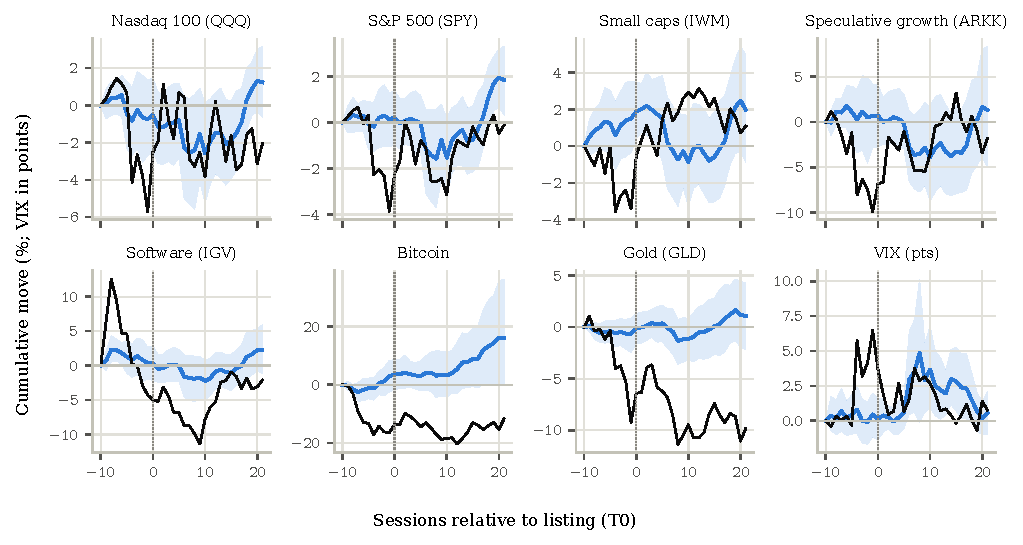
\includegraphics[width=\linewidth]{figures/f6_xasset.pdf}
\caption{Average cumulative move from the close 11 sessions before listing (blue, with 90\% bootstrap band across events) and SpaceX alone (black).}\label{fig:xasset}
\end{figure}

\begin{table}[!htbp]\centering\footnotesize
\caption{Cross-asset moves around 11 large US listings}\label{tab:xasset}

\begin{threeparttable}
\begin{tabular}{lrrrrrr}
\toprule
Asset & T$-$10 to T$-$1 & Listing day & T+1 to T+5 & T+6 to T+20 & Median T+1--5 & min $q$ \\
\midrule
S\&P 500 (SPY) & +0.2 & $-$0.2 & $-$1.2$^{**}$ & +3.1$^{**}$ & +0.3 & 0.48 \\
Nasdaq 100 (QQQ) & $-$0.5 & $-$0.6 & $-$1.1$^{*}$ & +3.8$^{*}$ & +0.3 & 0.48 \\
Small caps (IWM) & +1.9 & +0.1 & $-$1.8$^{**}$ & +1.9 & $-$0.7 & 0.48 \\
Speculative growth (ARKK) & +0.7 & $-$0.5 & $-$2.8$^{*}$ & +4.2 & $-$4.0 & 0.48 \\
Semis (SMH) & $-$1.1 & $-$0.6 & $-$1.2 & +5.9 & $-$1.2 & 0.48 \\
Software (IGV) & +0.3 & $-$0.7 & $-$1.2 & +4.2$^{*}$ & $-$0.7 & 0.48 \\
Bitcoin & +3.6 & +0.1 & +0.4 & +10.5 & +0.1 & 0.48 \\
Gold (GLD) & $-$0.1 & 0.0 & $-$0.1 & +1.1 & +0.5 & 0.83 \\
Long Treasuries (TLT) & $-$0.3 & $-$0.2 & +0.2 & $-$1.0 & +0.4 & 0.83 \\
Dollar (UUP) & +0.2 & +0.1 & +0.2 & $-$0.3 & +0.1 & 0.61 \\
High yield (HYG) & +0.2 & 0.0 & $-$0.5$^{**}$ & +0.9 & $-$0.2 & 0.48 \\
VIX (points) & +0.1 & +0.3 & +2.6$^{**}$ & $-$2.4 & +0.1 & 0.48 \\
US 10Y (bp) & +3.0 & +1.2 & $-$2.0 & +7.4 & $-$1.5 & 0.77 \\
Recent IPOs (IPO ETF) & +1.3 & $-$0.5 & $-$1.6 & +2.7 & +0.9 & 0.61 \\
\bottomrule
\end{tabular}
\begin{tablenotes}[flushleft]\footnotesize
\item \textit{Notes:} Average across events; percent except VIX (points) and US 10Y (basis points). Stars from a permutation test against 10,000 draws of 11 random dates since mid-2020 ($^{*}p<0.10$, $^{**}p<0.05$). min $q$ is the smallest Benjamini--Hochberg $q$ across the asset's four windows (56 tests in total); none is below 0.30.
\end{tablenotes}
\end{threeparttable}

\end{table}

\begin{table}[!htbp]\centering\scriptsize
\caption{Cross-asset trades around large listings}\label{tab:xtrades}

\begin{threeparttable}
\begin{tabular}{llrrrrrr}
\toprule
Asset & Trade & Mean & vs typical & Hit & $p$ & SR$_\text{event}$ & SR$_\text{real}$ \\
\midrule
Bitcoin & Short T-10 to T-1 & $-$3.6 & $-$1.5 & 45 & 0.67 & $-$0.33 & $-$0.44 \\
Bitcoin & Long T+1 to T+5 & +0.4 & $-$0.6 & 55 & 0.79 & 0.07 & 0.09 \\
Bitcoin & Long T+6 to T+20 & +10.5 & +7.4 & 82 & 0.11 & 0.37 & 0.49 \\
Speculative growth (ARKK) & Short T-10 to T-1 & $-$0.7 & $-$0.1 & 45 & 0.97 & $-$0.10 & $-$0.13 \\
Speculative growth (ARKK) & Long T+1 to T+5 & $-$2.8 & $-$3.0 & 45 & 0.095 & $-$0.46 & $-$0.61 \\
Speculative growth (ARKK) & Long T+6 to T+20 & +4.2 & +3.5 & 73 & 0.27 & 0.38 & 0.50 \\
Gold (GLD) & Short T-10 to T-1 & +0.1 & +0.7 & 45 & 0.51 & 0.02 & 0.03 \\
Gold (GLD) & Long T+1 to T+5 & $-$0.1 & $-$0.4 & 55 & 0.63 & $-$0.03 & $-$0.04 \\
Gold (GLD) & Long T+6 to T+20 & +1.1 & +0.3 & 55 & 0.83 & 0.24 & 0.32 \\
Nasdaq 100 (QQQ) & Short T-10 to T-1 & +0.5 & +1.4 & 55 & 0.26 & 0.12 & 0.16 \\
Nasdaq 100 (QQQ) & Long T+1 to T+5 & $-$1.1 & $-$1.5 & 55 & 0.087 & $-$0.27 & $-$0.36 \\
Nasdaq 100 (QQQ) & Long T+6 to T+20 & +3.8 & +2.6 & 73 & 0.083 & 0.81 & 1.07 \\
Semis (SMH) & Short T-10 to T-1 & +1.1 & +2.7 & 73 & 0.17 & 0.14 & 0.19 \\
Semis (SMH) & Long T+1 to T+5 & $-$1.2 & $-$2.0 & 45 & 0.16 & $-$0.17 & $-$0.23 \\
Semis (SMH) & Long T+6 to T+20 & +5.9 & +3.7 & 82 & 0.11 & 0.79 & 1.05 \\
Software (IGV) & Short T-10 to T-1 & $-$0.3 & +0.3 & 36 & 0.86 & $-$0.06 & $-$0.08 \\
Software (IGV) & Long T+1 to T+5 & $-$1.2 & $-$1.5 & 45 & 0.21 & $-$0.28 & $-$0.38 \\
Software (IGV) & Long T+6 to T+20 & +4.2 & +3.4 & 82 & 0.077 & 0.52 & 0.70 \\
Recent IPOs (IPO ETF) & Short T-10 to T-1 & $-$1.3 & $-$0.8 & 36 & 0.69 & $-$0.23 & $-$0.31 \\
Recent IPOs (IPO ETF) & Long T+1 to T+5 & $-$1.6 & $-$1.8 & 55 & 0.22 & $-$0.27 & $-$0.36 \\
Recent IPOs (IPO ETF) & Long T+6 to T+20 & +2.7 & +2.2 & 82 & 0.36 & 0.33 & 0.45 \\
\bottomrule
\end{tabular}
\begin{tablenotes}[flushleft]\footnotesize
\item \textit{Notes:} Percent per event, 11 events. ``vs typical'' subtracts the average of all same-length windows. SR$_\text{real}$ scales by $\sqrt{1.8}$ listings per year.
\end{tablenotes}
\end{threeparttable}

\end{table}

\begin{table}[!htbp]\centering\small
\caption{Abnormal return of other assets in the hour an IPO opens}\label{tab:hour}

\begin{threeparttable}
\begin{tabular}{lrrrrrr}
\toprule
Asset & \multicolumn{3}{c}{Large deals ($n=4$)} & \multicolumn{2}{c}{All ($n=14$)} & SpaceX \\ \cmidrule(lr){2-4}\cmidrule(lr){5-6} & bp & \% down & $t$ & bp & \% down & bp \\
\midrule
QQQ & $-$22 & 100\% & $-$2.8 & $-$6 & 71\% & $-$41 \\
SPY & $-$23 & 100\% & $-$2.2 & $-$5 & 57\% & $-$42 \\
Bitcoin & $-$21 & 75\% & $-$1.2 & $-$6 & 50\% & $-$50 \\
Gold (GLD) & $-$3 & 50\% & $-$0.0 & $-$1 & 50\% & $-$18 \\
ARKK & $-$51 & 75\% & $-$2.3 & $-$19 & 64\% & $-$82 \\
IWM & $-$32 & 100\% & $-$3.2 & $+$3 & 36\% & $-$51 \\
\bottomrule
\end{tabular}
\begin{tablenotes}[flushleft]\footnotesize
\item \textit{Notes:} Return in the IPO's first trading hour minus the average of the same clock hour over the prior 20 sessions, in basis points. Large deals: proceeds of \$1.4bn or more (CoreWeave, Medline, SpaceX, Venture Global).
\end{tablenotes}
\end{threeparttable}

\end{table}


\section{Application: the Anthropic listing}

Anthropic filed an amended S-1 on 10 November 2026 with a range of \$70--78 for 825 million Class~A shares, implying gross proceeds of about \$58--64bn. Press estimates put the implied market value at \$1.33--1.40tn, which makes the float about 4.4--4.6\%, similar to SpaceX's 4.2\% (4.8\% with the greenshoe). The company reports run-rate revenue of about \$81bn, so the implied value is roughly 16--17 times run-rate revenue, against about 39 times forward sales for SpaceX. Pricing is expected after the close on 18 November and trading on 19 November. The lock-up allows up to 10\% early sales by some holders and releases the rest over a staggered schedule of more than 20 windows. These terms come from secondary summaries of the filing and should be checked against the S-1/A itself.

\paragraph{Where it lists.} Anthropic lists into a backdrop that the cohort has not seen. The 10-year yield is 5.15\%, up 46bp in three months; the VIX is 19.3; fed funds are 3.88\%, up 25bp in six months. The 14-session run-up has been unusual but not extreme (Table~\ref{tab:runup}; Figure~\ref{fig:runup}): semiconductors, software and Bitcoin sit at their 6th to 8th percentiles, about 1.2 to 1.6 standard deviations below normal. The Q3 2026 IPO class was weak, with 30\% of deals pricing below range and the ten largest averaging $-6\%$ from the offer \citep{renaissance2026}.

\begin{figure}[!htbp]\centering
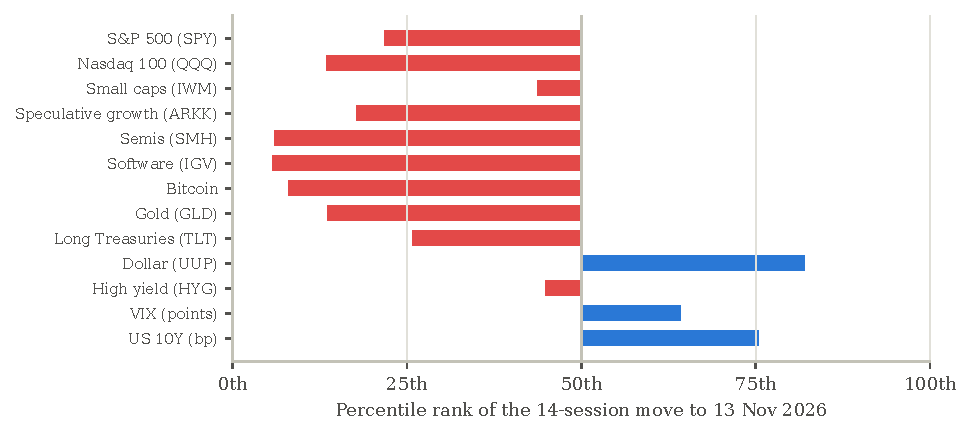
\includegraphics[width=0.85\linewidth]{figures/f7_runup.pdf}
\caption{Percentile rank of each asset's 14-session move to 13 November 2026, against every 14-session window since mid-2020.}\label{fig:runup}
\end{figure}

\begin{table}[!htbp]\centering\footnotesize
\caption{How unusual is the run-up to Anthropic?}\label{tab:runup}

\begin{threeparttable}
\begin{tabular}{lrrr}
\toprule
Asset & 14-session move & Percentile & $z$ \\
\midrule
S\&P 500 (SPY) & $$-$$1.4 & 22 & $-$0.67 \\
Nasdaq 100 (QQQ) & $$-$$4.5 & 13 & $-$1.16 \\
Small caps (IWM) & $+$0.2 & 44 & $-$0.12 \\
Speculative growth (ARKK) & $$-$$8.4 & 18 & $-$0.91 \\
Semis (SMH) & $$-$$10.1 & 6 & $-$1.59 \\
Software (IGV) & $$-$$9.2 & 6 & $-$1.59 \\
Bitcoin & $$-$$14.7 & 8 & $-$1.16 \\
Gold (GLD) & $$-$$3.4 & 14 & $-$1.01 \\
Long Treasuries (TLT) & $$-$$2.4 & 26 & $-$0.64 \\
Dollar (UUP) & $+$1.7 & 82 & $+$0.95 \\
High yield (HYG) & $+$0.2 & 45 & $-$0.04 \\
VIX (points) & $+$0.9 & 64 & $+$0.21 \\
US 10Y (bp) & $+$16.8 & 75 & $+$0.64 \\
Recent IPOs (IPO ETF) & $$-$$3.6 & 27 & $-$0.53 \\
\bottomrule
\end{tabular}
\begin{tablenotes}[flushleft]\footnotesize
\item \textit{Notes:} Move over the 14 sessions to 13 November 2026, ranked against every 14-session window since mid-2020.
\end{tablenotes}
\end{threeparttable}

\end{table}


\paragraph{A conditional plan.} The demand result suggests waiting for the pricing (Table~\ref{tab:tree}). A price above \$78 would place Anthropic in the group that popped most and gave back most; the conditional fade from day 5 to day 63 is the best historical setup available. A price within or below the range removes that edge; the cohort's median day-63 return in that group was positive. The calendar in Table~\ref{tab:cal} maps the horizons used in this note to dates. SpaceX's 8 December lock-up expiry falls on Anthropic's day 13, a potential overlap in supply.

\begin{table*}[!htbp]\centering\footnotesize
\caption{Conditional outlook by Anthropic's pricing}\label{tab:tree}

\begin{threeparttable}
\begin{tabular}{lrrrrrp{5.2cm}}
\toprule
Anthropic prices\ldots & $n$ & Pop & D21 & D63 & D126 & Historical edge (no allocation) \\
\midrule
Above \$78 (above range) & 28 & +32 & $-$2 & $-$20 & $-$27 & Fade day 5$\to$63: +11.5\%, hit 71\%, $p_W=0.028$ \\
\$70--78 or below & 14 & +4 & +1 & +14 & +7 & No reliable fade \\
\bottomrule
\end{tabular}
\begin{tablenotes}[flushleft]\footnotesize
\item \textit{Notes:} Cohort medians in percent for the two demand groups. Anthropic's range is \$70--78 for 825 million shares.
\end{tablenotes}
\end{threeparttable}

\end{table*}

\begin{table}[!htbp]\centering\small
\caption{Anthropic event calendar}\label{tab:cal}

\begin{threeparttable}
\begin{tabular}{llr}
\toprule
Event & Trading day & Date \\
\midrule
Pricing (after the close) & T$-$1 & Wed 18 Nov 2026 \\
Day 1: first trade & Day 1 & Thu 19 Nov 2026 \\
Day 5 & Day 5 & Wed 25 Nov 2026 \\
Day 13: SpaceX lock-up expiry & Day 13 & Tue 08 Dec 2026 \\
Day 21 & Day 21 & Fri 18 Dec 2026 \\
Day 63 & Day 63 & Mon 22 Feb 2027 \\
Day 126 (about 180 days) & Day 126 & Fri 21 May 2027 \\
\bottomrule
\end{tabular}
\begin{tablenotes}[flushleft]\footnotesize
\item \textit{Notes:} Day 1 = first close (19 November 2026). NYSE holidays applied (Thanksgiving, Christmas, New Year, MLK, Presidents' Day, Good Friday). SpaceX's 8 December lock-up expiry is Anthropic's day 13.
\end{tablenotes}
\end{threeparttable}

\end{table}


\paragraph{Scenarios.} Combining these results, we put roughly 50\% on a SpaceX-like path: a pop of 15--35\%, a peak in days 2--5, a 10--20\% decline from the first close by day 21, and a price near the offer by day 63. We put about 20\% on a bull case in which a strong first week persists, which would require yields to stop rising. We put about 30\% on a bear case in which an above-range pricing pops and then fades below the offer within three weeks. These probabilities are judgments informed by the statistics, not model outputs.

\section{Robustness and limitations}

\begin{itemize}
\item \textbf{Sample.} The cohort is hand-selected and small. It over-represents large, well-known deals, contains no 2022 listings, and has only one IPO valued above \$100bn (SpaceX). Conclusions about mega-caps rest on very few observations.
\item \textbf{Dependence.} IPOs cluster in hot windows \citep{lowry2002}, so returns are cross-sectionally correlated and effective sample sizes are smaller than the counts suggest. Reported $p$-values are optimistic even before correction.
\item \textbf{Overlapping windows.} An earlier version of this analysis found a strong correlation between first-week and three-month returns; it disappeared once the windows were made non-overlapping (Table~\ref{tab:corr}).
\item \textbf{Event study.} Eleven events cannot separate IPO effects from contemporaneous macro news, as the CoreWeave episode shows. Leave-one-out ranges and medians are reported for this reason.
\item \textbf{Costs.} Strategy returns ignore borrowing costs, which can be high and volatile for newly listed stocks, and ignore that options typically list a few days after the IPO.
\item \textbf{Data.} Market values at offer use shares outstanding where disclosed and reported valuations otherwise; hourly analysis drops IPOs whose feed omits the debut session (eToro, SK hynix).
\end{itemize}

\section{Conclusion}

The ``frenzy then fade'' description of IPOs is right on average and weak statistically. The frenzy is concentrated in the first day and the first hour of trading; the fade is slow, builds over three to six months, and is clearest relative to the Nasdaq. The only cross-sectional variable that reliably predicts outcomes is demand: hot deals pop more and give back more. Market value, sector, season, rates and float are reasonable priors but not signals. We find no systematic cross-asset liquidity drain before large listings. For Anthropic, the most useful single piece of information arrives on 18 November with the pricing; the best historical setup without an allocation carries a per-trade Sharpe ratio of about 0.4, which for a single name means low confidence.

\vspace{1em}
\noindent{\footnotesize\textit{Disclaimer.} This note is for research and discussion. It is not investment advice or a recommendation to buy or sell any security. Figures for Anthropic are based on public filings and press reports as of 15 November 2026 and may change.}

\bibliographystyle{plainnat}
\bibliography{refs}

\clearpage
\appendix
\section{Appendix}
\begin{table}[!htbp]\centering\small
\caption{Large-listing events used in the cross-asset study}\label{tab:events}

\begin{threeparttable}
\begin{tabular}{llr}
\toprule
Listing date & Company & Proceeds (\$bn) \\
\midrule
2020-09-16 & Snowflake & 3.4 \\
2020-12-09 & DoorDash + Airbnb & 6.9 \\
2021-03-11 & Coupang & 4.6 \\
2021-07-29 & Robinhood & 2.1 \\
2021-11-10 & Rivian & 11.9 \\
2023-09-14 & Arm & 4.9 \\
2024-07-25 & Lineage & 4.4 \\
2025-03-28 & CoreWeave & 1.5 \\
2025-12-17 & Medline & 6.3 \\
2026-06-12 & SpaceX & 75 \\
2026-07-10 & SK hynix ADR & 26.5 \\
\bottomrule
\end{tabular}
\begin{tablenotes}[flushleft]\footnotesize
\item \textit{Notes:} DoorDash and Airbnb listed one day apart and are treated as one event. SK hynix is a cross-listing of an already-public company.
\end{tablenotes}
\end{threeparttable}

\end{table}

\begin{scriptsize}\setlength{\tabcolsep}{2.6pt}
\begin{longtable}{llllrrrrlrrr}
\caption{The IPO cohort}\label{tab:cohort}\\
\toprule
Company & Ticker & Listed & Sector & Offer & Cap \$bn & Proceeds \$m & Float \% & vs range & Pop & D21 & D63 \\
\midrule
\endfirsthead
\toprule Company & Ticker & Listed & Sector & Offer & Cap \$bn & Proceeds \$m & Float \% & vs range & Pop & D21 & D63 \\ \midrule
\endhead
\bottomrule \multicolumn{12}{l}{\scriptsize Returns in percent; D21/D63 from the day-1 close. Sources: SEC 424B4, company pricing releases, Yahoo Finance.} \\ \endlastfoot
Snowflake & SNOW & 2020-09-16 & Software & 120 & 33.3 & 3,360 & 10.1 & Above & +112 & $-$4 & +30 \\
Unity & U & 2020-09-18 & Software & 52 & 20.3 & 1,300 & 6.4 & Above & +31 & +35 & +115 \\
DoorDash & DASH & 2020-12-09 & Consumer internet & 102 & 38.3 & 3,366 & 8.8 & Above & +86 & $-$18 & $-$24 \\
Airbnb & ABNB & 2020-12-10 & Consumer internet & 68 & 47.3 & 3,490 & 7.4 & Above & +113 & +2 & +43 \\
Affirm & AFRM & 2021-01-13 & Fintech & 49 & 12.5 & 1,205 & 9.6 & Above & +97 & +45 & $-$29 \\
Bumble & BMBL & 2021-02-11 & Consumer internet & 43 & 8.2 & 2,150 & 26.2 & Above & +64 & $-$1 & $-$33 \\
Oscar Health & OSCR & 2021-03-03 & Fintech & 39 & 7.6 & 1,419 & 18.7 & Above & $-$11 & $-$23 & $-$27 \\
Coupang & CPNG & 2021-03-11 & Consumer internet & 35 & 64.2 & 4,550 & 7.1 & Above & +41 & $-$7 & $-$23 \\
Compass & COMP & 2021-04-01 & Consumer internet & 18 & 3.0 & 450 & 15.0 & Below & +12 & $-$6 & $-$35 \\
Duolingo & DUOL & 2021-07-28 & Software & 102 & 4.0 & 521 & 13.0 & Above & +32 & $-$5 & +40 \\
Robinhood & HOOD & 2021-07-29 & Fintech & 38 & 32.0 & 2,090 & 6.5 & Within & $-$8 & +35 & +14 \\
Toast & TOST & 2021-09-22 & Software & 40 & 20.0 & 870 & 4.3 & Above & +56 & $-$18 & $-$45 \\
Rivian & RIVN & 2021-11-10 & Industrials & 78 & 66.0 & 11,934 & 18.1 & Above & +29 & +15 & $-$36 \\
Nextracker & NXT & 2023-02-09 & Industrials & 24 & 3.5 & 638 & 18.2 & Above & +27 & +2 & +9 \\
Cava & CAVA & 2023-06-15 & Consumer & 22 & 2.5 & 318 & 13.0 & Above & +99 & +9 & $-$18 \\
Arm & ARM & 2023-09-14 & Software & 51 & 54.5 & 4,870 & 8.9 & Within & +25 & $-$18 & +2 \\
Instacart & CART & 2023-09-19 & Consumer internet & 30 & 10.0 & 660 & 6.6 & Above & +12 & $-$27 & $-$27 \\
Klaviyo & KVYO & 2023-09-20 & Software & 30 & 9.2 & 576 & 6.3 & Above & +9 & $-$6 & $-$14 \\
Birkenstock & BIRK & 2023-10-11 & Consumer & 46 & 8.1 & 1,484 & 18.2 & Within & $-$13 & +5 & +19 \\
Astera Labs & ALAB & 2024-03-20 & Software & 36 & 5.4 & 713 & 13.2 & Above & +72 & +14 & +8 \\
Reddit & RDDT & 2024-03-21 & Consumer internet & 34 & 4.9 & 748 & 15.3 & Within & +48 & $-$19 & +14 \\
Ibotta & IBTA & 2024-04-19 & Consumer & 88 & 2.7 & 577 & 21.7 & Above & +11 & +8 & $-$34 \\
Rubrik & RBRK & 2024-04-25 & Software & 32 & 5.6 & 752 & 13.4 & Above & +16 & $-$11 & $-$7 \\
Viking & VIK & 2024-05-01 & Consumer & 24 & 10.4 & 1,537 & 14.8 & Within & +9 & +17 & +37 \\
Waystar & WAY & 2024-06-07 & Healthcare & 21.5 & 3.7 & 968 & 26.1 & Within & $-$4 & 0 & +32 \\
Tempus AI & TEM & 2024-06-14 & Healthcare & 37 & 6.2 & 411 & 6.7 & Within & +9 & +1 & +23 \\
Lineage & LINE & 2024-07-25 & Industrials & 78 & 19.6 & 4,437 & 22.6 & Above & +4 & +5 & $-$2 \\
StandardAero & SARO & 2024-10-02 & Industrials & 24 & 8.0 & 1,440 & 17.9 & Above & +36 & $-$10 & $-$24 \\
Venture Global & VG & 2025-01-24 & Industrials & 25 & 60.5 & 1,750 & 2.9 & Below & $-$4 & $-$37 & $-$64 \\
SailPoint & SAIL & 2025-02-13 & Software & 23 & 12.8 & 1,380 & 10.8 & Within & $-$4 & $-$15 & $-$14 \\
CoreWeave & CRWV & 2025-03-28 & Software & 40 & 23.0 & 1,500 & 6.5 & Below & 0 & +5 & +300 \\
eToro & ETOR & 2025-05-13 & Fintech & 52 & 4.2 & 620 & 14.8 & Above & 0 & +21 & $-$2 \\
Hinge Health & HNGE & 2025-05-22 & Healthcare & 32 & 2.6 & 437 & 16.8 & Within & +17 & +16 & +49 \\
Circle & CRCL & 2025-06-05 & Fintech & 31 & 6.8 & 1,054 & 15.5 & Above & +168 & +149 & +41 \\
Chime & CHYM & 2025-06-12 & Fintech & 27 & 11.6 & 864 & 7.4 & Above & +37 & $-$19 & $-$35 \\
Figma & FIG & 2025-07-31 & Software & 33 & 19.3 & 1,219 & 6.3 & Above & +250 & $-$38 & $-$55 \\
Figure & FIGR & 2025-09-11 & Fintech & 25 & 5.3 & 788 & 14.9 & Above & +24 & +54 & +30 \\
Klarna & KLAR & 2025-09-11 & Fintech & 40 & 15.1 & 1,372 & 9.1 & Above & +7 & $-$3 & $-$28 \\
Gemini & GEMI & 2025-09-12 & Fintech & 28 & 3.3 & 425 & 12.8 & Above & +14 & $-$27 & $-$65 \\
StubHub & STUB & 2025-09-17 & Consumer internet & 23.5 & 8.6 & 800 & 9.3 & Within & $-$6 & $-$12 & $-$36 \\
Netskope & NTSK & 2025-09-18 & Software & 19 & 7.3 & 908 & 12.4 & Above & +18 & +1 & $-$11 \\
Medline & MDLN & 2025-12-17 & Healthcare & 29 & 40.0 & 6,265 & 15.7 & Within & +41 & +8 & +6 \\
SpaceX & SPCX & 2026-06-12 & Industrials & 135 & 1,770.0 & 75,000 & 4.2 & -- & +19 & $-$15 & $-$6 \\
\end{longtable}
\end{scriptsize}


\end{document}
